\documentclass{beamer}
\usepackage[latin1]{inputenc}
\usetheme{Warsaw}
\title{Introduction to Nuclear Magnetic Resonance Spectroscopy}
\author{Dr Alexey Potapov}
\institute{University of Nottingham, School of Physics and Astronomy}
\date{Jule 13, 2017}

\setbeamertemplate{headline}{}
\setbeamertemplate{footline}{}
\setbeamertemplate{caption}{Fig.\insertcaptionnumber: \insertcaption \par}
\setbeamerfont{caption}{size=\scriptsize }
%\newenvironment{slide}[1]
%{\begin{frame}[environment=slide]
%		\frametitle{\insertsection-#1}}
%	{\end{frame}}


\begin{document}
	
	
	
	\begin{frame}
		\titlepage
	\end{frame}
	
	\section{Introduction. Magnetic moment in magnetic field.}
	\subsection{Introduction to Magnetic Resonance}	
	\begin{frame}{\thesection.\thesubsection. \insertsubsection}

		
		\begin{itemize}
		\item Magnetic resonance (MR) is a phenomenon of resonant energy absorption by a system of nuclei (and electrons). 
		\item Nuclear magnetic resonance (NMR) results from the intrinsic magnetic moment of the
		nuclei of some atoms. Magnetic moments of electrons are exploited in electron spin resonance.
		\item Magnetic resonance (MR) generally involves placing a sample in a strong magnetic
		field (to generate polarisation at a fixed resonant frequency) and detecting signals
		produced following application of pulsed radio-frequency electromagnetic fields (RF
		pulses).
		\item MR is a very powerful method for studying the structure of materials: used in physics, chemistry, biology, medicine etc.

		\end{itemize}
	\end{frame}
	
	\subsection{Applications of NMR}
	
	  	
	
	\begin{frame}{\thesection.\thesubsection. \insertsubsection}
	
	 \begin{itemize}
	 	\item NMR spectroscopy is used for chemical analysis and for molecular structure determination	  	
	 \end{itemize}
	 
	
		
		\begin{figure}[ht]
			\begin{minipage}[t]{0.45\linewidth}
				\centering
				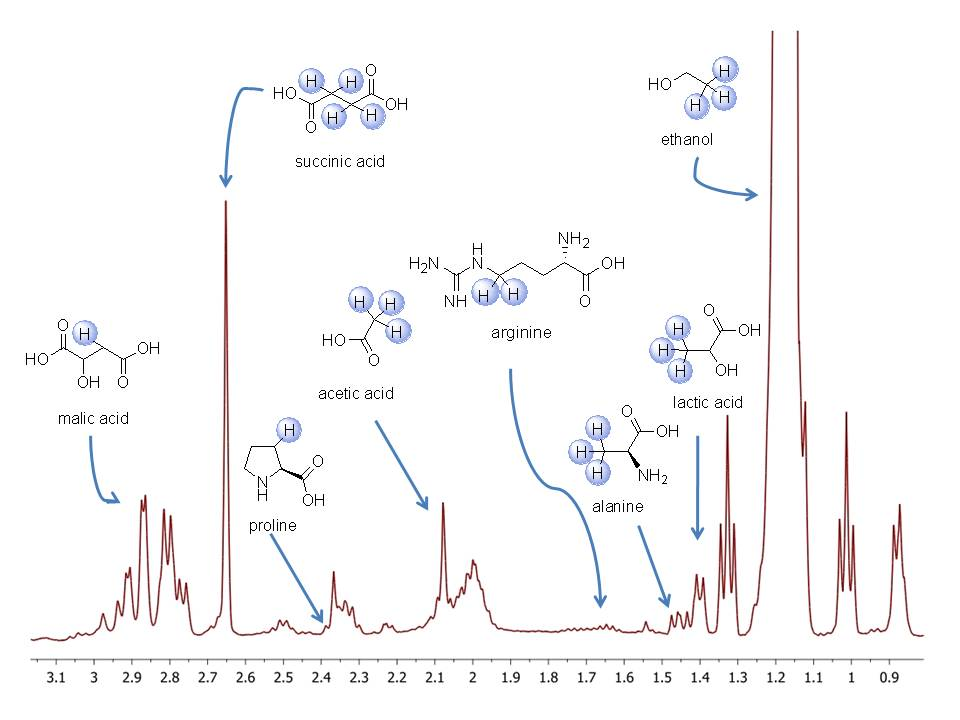
\includegraphics[width=\textwidth]{wine_spectrum.jpg}
				\caption{\textsuperscript{1}H NMR spectrum of a sample of Spanish wine (\url{http://www.unirioja.es/gsoe/NMR.htm})}
				\label{fig1}
			\end{minipage}
			\hspace{0.3cm}
			\begin{minipage}[t]{0.45\linewidth}
				\centering
				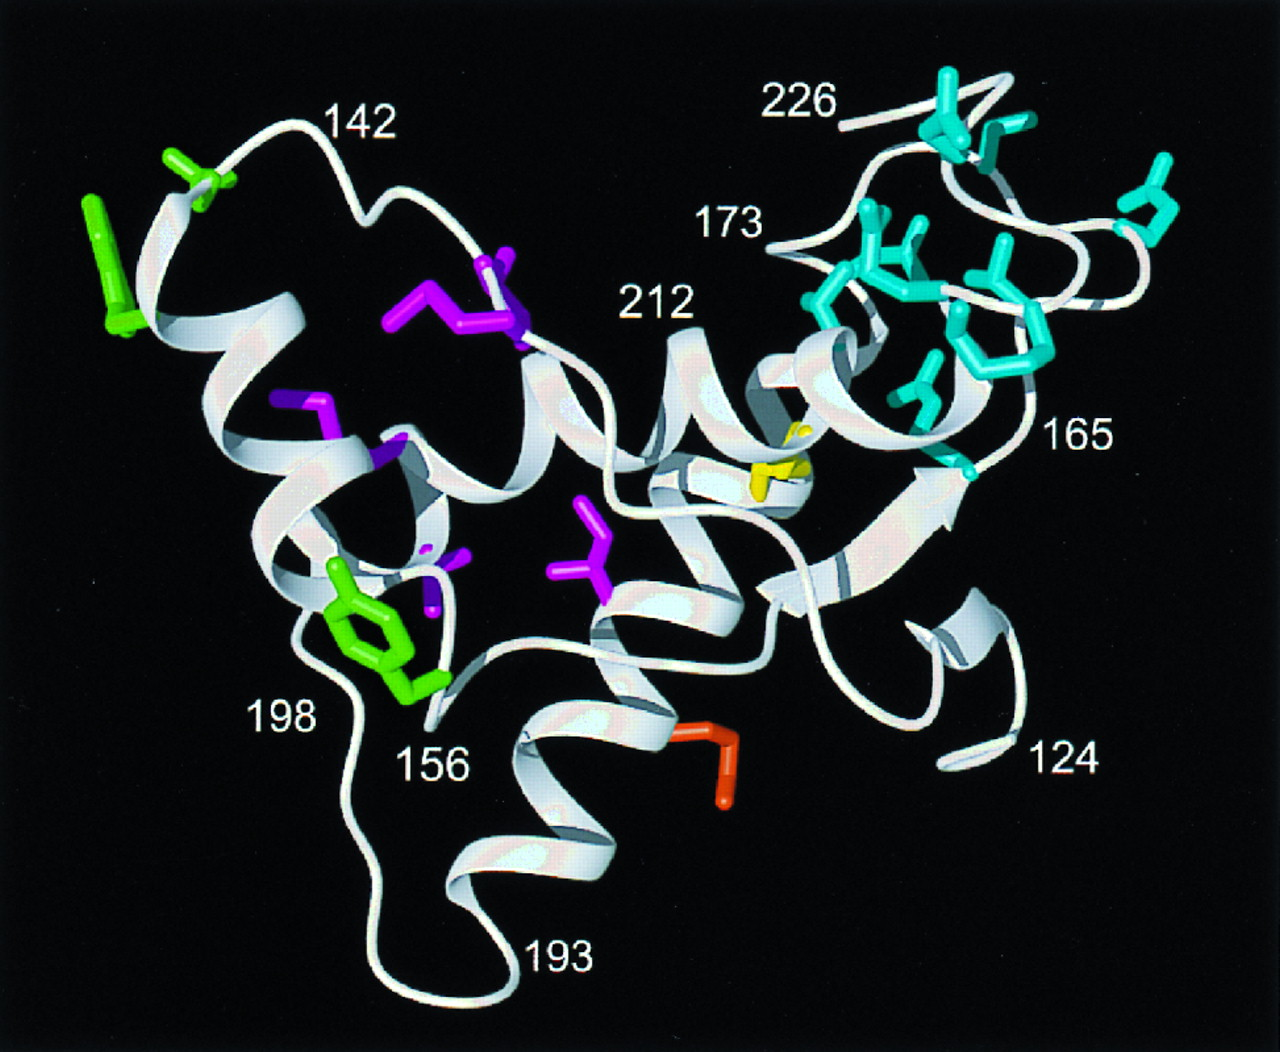
\includegraphics[width=\textwidth]{prion.jpg}
				\caption{NMR-derived structure of a prion  \url{http://www.pnas.org/content/94/14/7281.full}}
				\label{fig3}
			\end{minipage}					
		\end{figure}
	\end{frame}
	
	
	\begin{frame}{\thesection.\thesubsection. \insertsubsection}
		\begin{itemize}
			\item NMR relaxometry can be used to monitor molecular environment
		\end{itemize}

		\begin{figure}[ht]
					
						
			\begin{minipage}[t]{0.15\textwidth}
				\centering
				(a)
				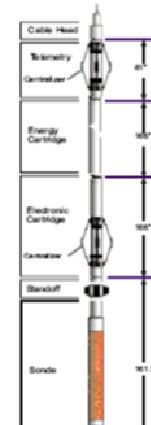
\includegraphics[width=\textwidth]{well_logging1.jpg}

			\end{minipage}
			\hspace{0.1cm}
			\begin{minipage}[t]{0.15\textwidth}
				\centering
				(b)
				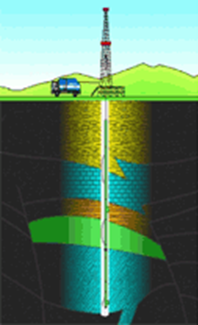
\includegraphics[width=\textwidth]{well_logging2.png}
				\label{fig7}
			\end{minipage}			
			\hspace{0.1cm}
			\begin{minipage}[t]{0.15\textwidth}
				\centering
				(c)
				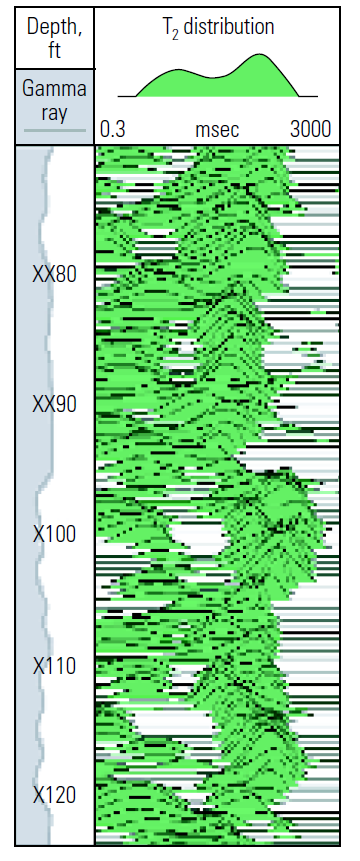
\includegraphics[width=\textwidth]{well_logging3.png}
				\label{fig5}
			\end{minipage}		
						\hspace{0.1cm}
		
				\caption{ (a) NMR-logging probe, (b) Schematic positioning of the probe in a well, (c) T\textsubscript{2}-relaxation profile along the bore. Sources: 1) Allenet al. Oilfield review, Autumn 2000; 2) Coates, Xiao NMR Logging Principles and Applications, Hulliburton}		
		\end{figure}			
	\end{frame}
	
\begin{frame}{\thesection.\thesubsection. \insertsubsection}
	\begin{itemize}
		\item NMR forms the basis for magnetic resonance imaging (MRI)
	\end{itemize}
	
	\begin{figure}[ht]
		
		
			\centering
		
			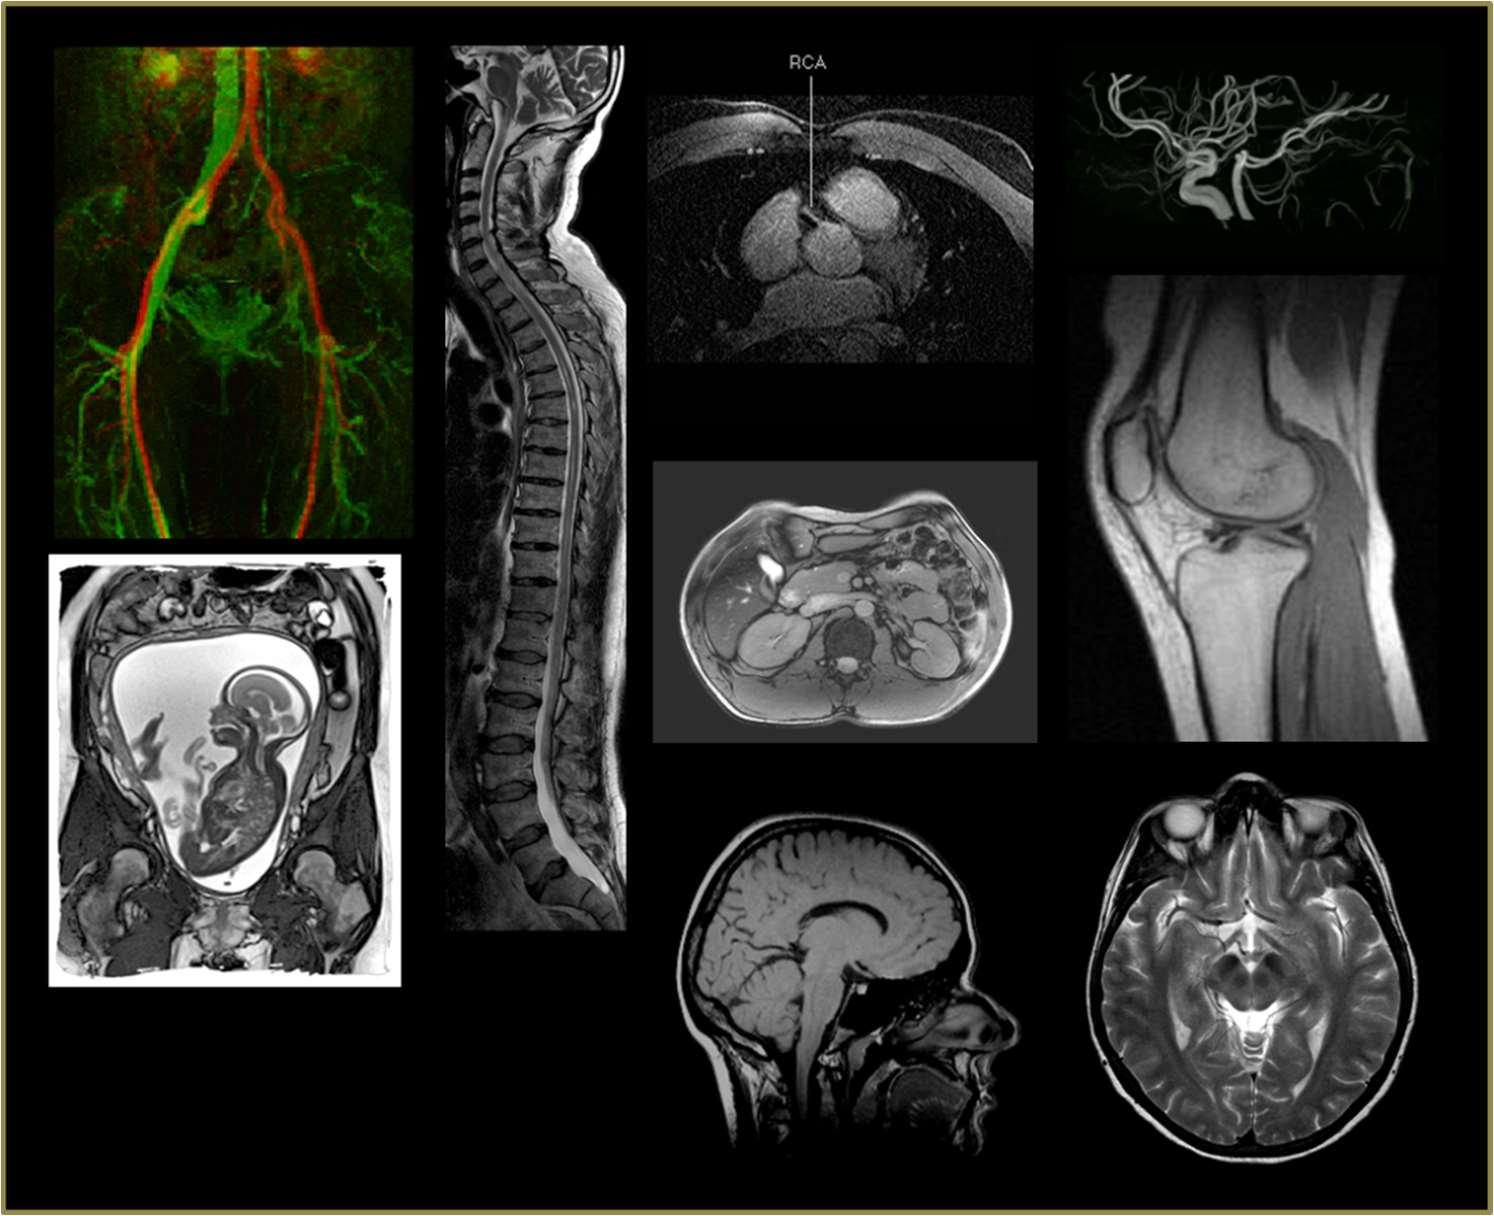
\includegraphics[width=0.7\textwidth]{mri.jpeg}
		
		\caption{  Example magnetic resonance images of blood vessel (in legs), fetus in utero, spine, heart, abdomen, head, blood vessels (in brain), knee, brain (courtesy of Prof. Richard Bowtell)}		
	\end{figure}			
\end{frame}

\end{document}